\subsection{Модель сверхширокоугольного объектива}

Сверхширокоугольные объективы имеют в своей основе сложную систему линз, схема которой представлена на рисунке \ref{pic:fyscheme}. 
Особенности этой системы позволяют достигать существенного угла обзора, но также являются причиной аберрации и характерных искажений 
изображения. 

\begin{figure}[H]
    \begin{center}
        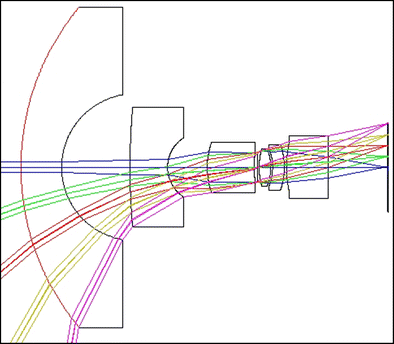
\includegraphics[scale=0.5]{pics/fisheye_scheme.png}                                                                                            %TODO: перерисовать схему?
        \caption{Системы кругового обзора}
        \label{pic:fyscheme}
    \end{center}
\end{figure}
    
Перед использованием снимков с подобных камер необходимо избавиться от искажений. Для осуществления этого необходима модель камеры - 
набор уравнений, который позволяет найти проекцию точки в мировых координатах на плоскость изображения и наоборот. Перспективная проекция, 
которая обычно используется для описания камер, не способна спроецировать широкоугольный снимок на кадр конечного размера. Поэтому при производстве
 fisheye-объективов опираются на другие виды проекций \ref{}. Но реальные линзы не всегда в точности следуют заданным моделям, по этой 
 причине для моделирования подобных искажений принято использовать многочлен вида

 \begin{equation}	% TODO: переписать уравнение 
	\begin{split}
        \begin{pmatrix}x_d\\y_d\end{pmatrix} = \frac{\theta}{r}\left[ 1 + k_1\theta^2 + k_2\theta^4 + k_3\theta^6 + k_4\theta^8\right]\begin{pmatrix}x_n\\y_n\end{pmatrix},
        \label{eqn:fisheye_distortion}
    \end{split}
\end{equation}

где $k_i$ - внутренние параметры камеры. 
% Стандартная для обычных камер модель камеры-обскуры хоть и способна учитывать радиальные искажения, не работает при таких больших углах зрения. 
В настоящий момент есть несколько распространённых моделей, аппроксимирующих реальные искажения подобных объективов. Модель Канналы и 
Брандта \cite{opencv_model} реализована в OpenCV и описывает радиальные искажения через угол падения луча света на линзу, а не расстояние  
от центра изображения до места падения, как это делалось в более ранних моделях. 

\begin{equation}	
        \theta = \arctan(\frac{r}{f})
        \label{eqn:kannala_theta}
\end{equation}

\begin{equation}	
    \delta r = k_1\theta + k_2\theta^3 + k_3\theta^5 + k_4\theta^7 + ... + k_n\theta^{n+1}
    \label{eqn:kannala_delta}
\end{equation}

\subsection{Обзор существующих систем стереозрения, использующих сверхширокоугольные изображения}

